\documentclass[11pt]{article}
\usepackage[T1]{fontenc}
\usepackage[utf8]{inputenc}
\usepackage{lmodern}
\usepackage[french]{babel}
\usepackage[a4paper,margin=2.4cm]{geometry}
\usepackage{amsmath,amssymb,amsthm,bm}
\usepackage{graphicx}
\usepackage{booktabs}
\usepackage[colorlinks=true,linkcolor=blue,citecolor=blue]{hyperref}
\usepackage[nameinlink,noabbrev]{cleveref}
\crefname{table}{tableau}{tableaux}
\graphicspath{{figures/}}

\theoremstyle{definition}
\newtheorem{proposition}{Proposition}
\theoremstyle{remark}
\newtheorem*{remarque}{Remarque}

\newcommand{\R}{\mathbb{R}}
\newcommand{\E}{\mathbb{E}}
\newcommand{\N}{\mathcal{N}}
\newcommand{\X}{\mathbf{X}}
\newcommand{\z}{\mathbf{z}}
\newcommand{\uu}{\mathbf{u}}
\newcommand{\wrap}{\operatorname{wrap}}
\newcommand{\diag}{\operatorname{diag}}
\newcommand{\Neff}{N_{\mathrm{eff}}}

\title{\bfseries Méthodes de Monte-Carlo : intégration et filtrage}
\author{Mohamed Benloughmari \and Fatimetou Narjah}
\date{\today}

\begin{document}
\maketitle

\begin{abstract}
Ce compte rendu réunit deux applications des méthodes de Monte-Carlo. On étudie
d'abord l'estimation d'intégrales par Monte-Carlo classique puis par
échantillonnage d'importance, en comparant leurs variances, leur vitesse de
convergence et en validant le théorème central limite. On aborde ensuite la
localisation d'un robot mobile par filtrage particulaire, en analysant
l'influence du nombre de particules, du nuage initial, des bruits du filtre,
d'une panne capteur et de la stratégie de rééchantillonnage.
\end{abstract}

% ======================================================================
% PARTIE 1 : Importance sampling
% ======================================================================

\section{Introduction}

L'objectif de ce TP est d'étudier différentes méthodes de Monte-Carlo pour
approximer une intégrale et de comparer leur précision ainsi que leur coût de
calcul.

On considère l'intégrale :
\[
\mu = \int_0^1 \cos\left(\frac{\pi x}{2}\right)\,dx.
\]
Sa valeur exacte est :
\[
\mu = \frac{2}{\pi} \approx 0{,}63662.
\]
Dans un premier temps, nous étudions la méthode de Monte-Carlo classique. Nous
considérons ensuite la méthode d'échantillonnage d'importance
(\textit{Importance Sampling}), qui consiste à utiliser une densité de
probabilité adaptée afin de réduire la variance de l'estimateur. Enfin, nous
comparons les résultats théoriques aux résultats obtenus par simulation
numérique, étudions la convergence des estimateurs et vérifions numériquement
le théorème central limite.

\section{Méthode de Monte-Carlo classique}

\subsection{Variance théorique}

Pour $X\sim\mathcal{U}([0,1])$ et $g(x)=\cos\left(\frac{\pi x}{2}\right)$, on
a :
\[
\mathbb{E}[g(X)]=\frac{2}{\pi},
\qquad
\mathbb{E}[g(X)^2]=\frac{1}{2}.
\]
Ainsi,
\[
\operatorname{Var}(g(X))
=\frac{1}{2}-\frac{4}{\pi^2}
\approx 0{,}094715.
\]
La variance de l'estimateur de Monte-Carlo est donc :
\[
\operatorname{Var}(\widehat{\mu}_N)
=\frac{1}{N}\left(\frac{1}{2}-\frac{4}{\pi^2}\right).
\]
Pour $N=50$, on obtient :
\[
\boxed{\operatorname{Var}(\widehat{\mu}_{50})
\approx 0{,}0018943.}
\]

\subsection{Estimation empirique de la variance}

Pour $N=50$, nous réalisons $M=100$ simulations indépendantes. La moyenne et la
variance empiriques des estimations sont :
\[
\overline{\mu}=0{,}638955,
\qquad
V_{\mathrm{emp}}=0{,}00141784.
\]
La variance théorique étant $V_{\mathrm{th}}=0{,}00189431$, on constate que la
variance empirique est du même ordre de grandeur, mais présente un écart dû aux
fluctuations aléatoires et au nombre limité de simulations.

\subsection{Étude de la convergence en fonction de $N$}

D'après la loi des grands nombres, l'estimateur $\widehat{\mu}_N$ converge vers
$\mu=2/\pi$ lorsque $N$ augmente. Le graphique compare l'erreur quadratique
moyenne (RMSE) empirique à l'erreur théorique :
\[
\operatorname{RMSE}(\widehat{\mu}_N)
=\sqrt{\frac{\operatorname{Var}(g(X))}{N}}.
\]

\begin{figure}[h]
    \centering
    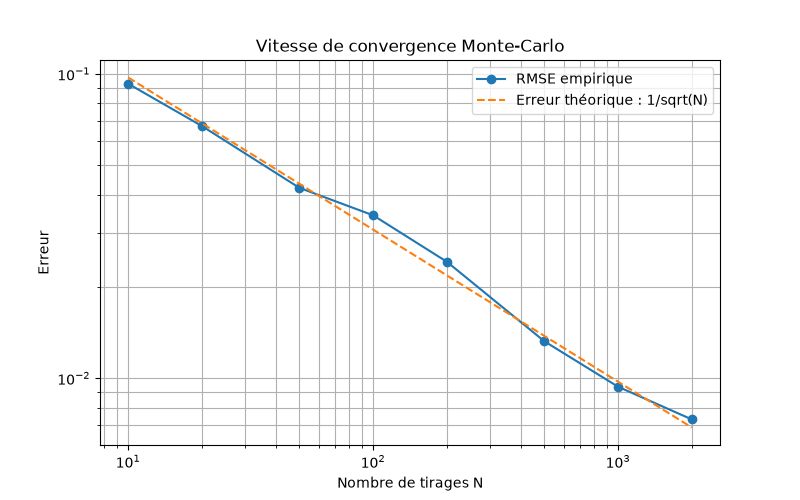
\includegraphics[width=0.85\textwidth]{convergence.png}
    \caption{Convergence de l'estimateur de Monte-Carlo en fonction du nombre de tirages $N$.}
    \label{fig:convergence}
\end{figure}

On observe que l'erreur diminue lorsque le nombre de tirages augmente et que la
courbe empirique suit globalement la courbe théorique. L'erreur évolue en
$1/\sqrt{N}$ : pour diviser l'erreur par deux, il faut multiplier $N$ par
quatre.

\subsection{Vérification numérique du TCL}

Pour $N=50$, nous réalisons $M=10\,000$ simulations indépendantes. Chaque
estimation est centrée et réduite :
\[
Z_N=\frac{\widehat{\mu}_N-\mu}
{\sqrt{\operatorname{Var}(g(X))/N}}.
\]
D'après le théorème central limite, $Z_N$ suit approximativement une loi
normale standard $\mathcal{N}(0,1)$.

La simulation donne :
\[
\mathbb{E}_{\mathrm{emp}}[Z_N]\approx -0{,}045,
\qquad
\operatorname{Var}_{\mathrm{emp}}(Z_N)\approx 0{,}850.
\]
L'histogramme obtenu présente une forme globalement en cloche, compatible avec
une approximation normale. La moyenne empirique est proche de $0$ et la
variance proche de $1$ ; les écarts observés sont dus aux fluctuations de la
simulation.

\begin{figure}[h]
    \centering
    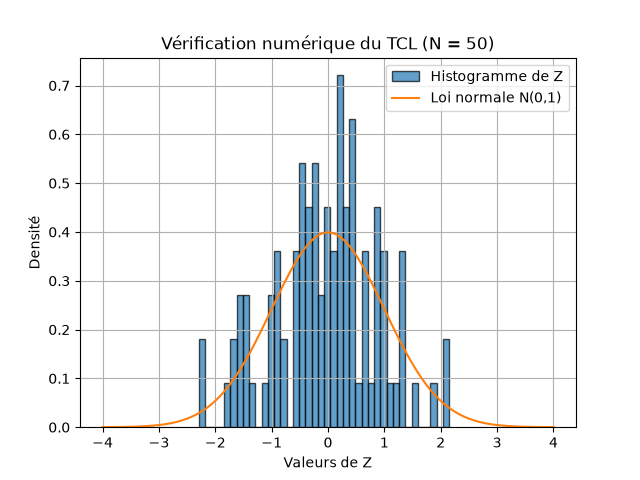
\includegraphics[width=0.8\textwidth]{tcl_monte_carlo.png}
    \caption{Vérification numérique du TCL pour Monte-Carlo classique avec $N=50$.}
    \label{fig:tcl-mc}
\end{figure}

\section{Importance sampling}

\subsection{Détermination de la densité d'importance optimale}

La densité d'importance optimale est proportionnelle à $g(x)q(x)$ et s'écrit :
\[
\boxed{
\widetilde q_{\mathrm{opt}}(x)
=\frac{g(x)q(x)}{\mu}
=\frac{\pi}{2}\cos\left(\frac{\pi x}{2}\right).
}
\]
Cette densité minimise la variance de l'estimateur. Elle n'est généralement pas
directement utilisable, car sa normalisation dépend de $\mu$, l'intégrale que
l'on cherche à estimer.

\subsection{Développement limité au voisinage de $0$}

Le développement limité de $\cos(u)$ au voisinage de $0$ est :
\[
\cos(u)=1-\frac{u^2}{2}+o(u^2).
\]
En prenant $u=\frac{\pi x}{2}$, on obtient :
\[
\boxed{
g(x)=\cos\left(\frac{\pi x}{2}\right)
=1-\frac{\pi^2x^2}{8}+o(x^2).
}
\]
Ainsi, une approximation au voisinage de $0$ est
$g(x)\approx 1-\frac{\pi^2x^2}{8}$.

\subsection{Validité de l'approximation comme densité}

On ne peut pas utiliser directement $1-\frac{\pi^2x^2}{8}$ comme densité sur
$[0,1]$, car une densité doit être positive ou nulle partout. Or, en $x=1$ :
\[
1-\frac{\pi^2}{8}<0.
\]
Cette approximation ne satisfait donc pas la condition de positivité d'une
densité.

\subsection{Normalisation de la densité proposée}

On considère une densité de la forme $\widetilde q(x)=C(1-x^2)$ sur $[0,1]$.
Pour qu'elle soit une densité de probabilité, il faut :
\[
\int_0^1 C(1-x^2)\,dx=1.
\]
Ainsi,
\[
C\left[x-\frac{x^3}{3}\right]_0^1=1
\quad\Longrightarrow\quad
C\frac{2}{3}=1.
\]
Par conséquent,
\[
\boxed{C=\frac{3}{2}},
\qquad
\boxed{\widetilde q(x)=\frac{3}{2}(1-x^2)}.
\]

\subsection{Tracé et comparaison des densités}

Nous traçons les trois fonctions $q(x)$, $g(x)q(x)$ et $\widetilde q(x)$ sur
$[0,1]$, avec :
\[
q(x)=1,\qquad
g(x)q(x)=\cos\left(\frac{\pi x}{2}\right),
\qquad
\widetilde q(x)=\frac{3}{2}(1-x^2).
\]
La densité uniforme $q(x)$ est constante, tandis que $g(x)q(x)$ et
$\widetilde q(x)$ sont décroissantes et s'annulent en $x=1$. La densité
d'importance proposée est plus élevée que $g(x)q(x)$ sur une grande partie de
l'intervalle. Elle permet ainsi de générer davantage d'échantillons près de
$x=0$, où $g(x)q(x)$ est élevée.

\begin{figure}[h]
    \centering
    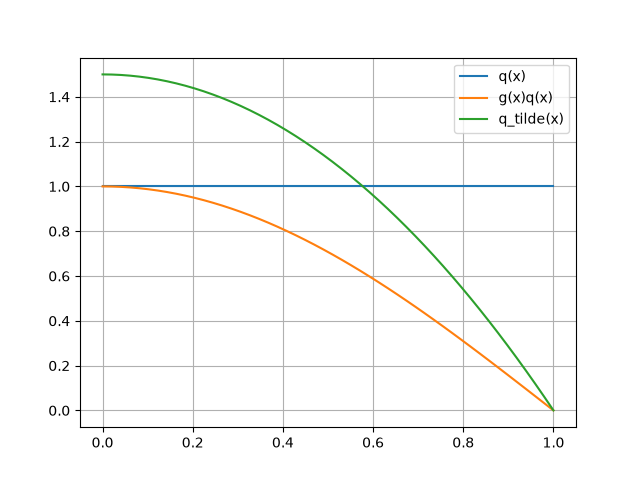
\includegraphics[width=0.8\textwidth]{densites.png}
    \caption{Comparaison de $q(x)$, $g(x)q(x)$ et $\widetilde q(x)$.}
    \label{fig:densites}
\end{figure}

\section{Importance sampling avec acceptation-rejet}

\subsection{Détermination de la densité d'importance}

Le développement limité de $g(x)=\cos(\pi x/2)$ au voisinage de $0$ donne :
\[
g(x)\approx 1-\frac{\pi^2x^2}{8}.
\]
Cette approximation peut devenir négative sur $[0,1]$. On propose donc une
densité de la forme $\widetilde q(x)=C(1-x^2)$, où $C$ est une constante. La
condition de normalisation impose :
\[
\int_0^1 C(1-x^2)\,dx=1
\quad\Longrightarrow\quad C=\frac32.
\]
La densité d'importance utilisée est donc :
\[
\boxed{\widetilde q(x)=\frac32(1-x^2).}
\]

\subsection{Calcul de la variance théorique}

L'estimateur d'importance sampling repose sur les poids
\[
H(x)=\frac{g(x)q(x)}{\widetilde q(x)}
=\frac{\cos(\pi x/2)}{\frac32(1-x^2)}.
\]
Sa variance théorique est :
\[
\operatorname{Var}(\widehat{\mu}_N)
=\frac{1}{N}
\left[
\int_0^1\frac{g(x)^2q(x)^2}{\widetilde q(x)}\,dx
-\mu^2
\right].
\]
L'intégrale est calculée numériquement avec Python. Pour $N=50$, on obtient :
\[
\boxed{
\operatorname{Var}(\widehat{\mu}_{50})
\approx 1{,}98166\times10^{-5}.
}
\]

\subsection{Méthode d'acceptation-rejet}

Pour générer des échantillons suivant la densité
$\widetilde q(x)=\frac32(1-x^2)$, on propose $X\sim\mathcal U([0,1])$ et
$U\sim\mathcal U([0,1])$, puis on accepte $X$ si :
\[
U<1-X^2.
\]
La probabilité d'acceptation théorique est :
\[
P_a=\frac{1}{3/2}\int_0^1
\frac32(1-x^2)\,dx
=\boxed{\frac23\approx 0{,}6667}.
\]
Pour $M=10^5$ propositions, la simulation donne :
\[
P_{a,\mathrm{emp}}=0{,}66903,
\qquad
\text{écart}=0{,}00236.
\]
Au total, $66\,903$ valeurs ont été acceptées. La probabilité empirique est
proche de la valeur théorique, ce qui valide numériquement la méthode
d'acceptation-rejet.

\subsection{Estimation empirique de la variance}

Nous réalisons $M=10\,000$ simulations indépendantes, avec $N=50$ échantillons
acceptés pour chaque estimation. La variance empirique est calculée à partir
des estimations $\widehat{\mu}_N^{(m)}$ :
\[
\widehat V_{\mathrm{emp}}
=\frac{1}{M-1}\sum_{m=1}^{M}
\left(\widehat{\mu}_N^{(m)}-\overline{\mu}\right)^2.
\]
Les résultats obtenus sont :
\[
\overline{\mu}=0{,}636624,
\qquad
\widehat V_{\mathrm{emp}}\approx 2{,}00982\times10^{-5}.
\]
La variance empirique est proche de la variance théorique
$1{,}98166\times10^{-5}$. Cela confirme la cohérence des résultats numériques.

\section{Comparaison des deux méthodes}

\subsection{Comparaison théorique et empirique des variances}

Pour $N=50$, les variances théoriques des deux méthodes sont :
\[
V_{\mathrm{MC}} \approx 1{,}8943\times10^{-3},
\qquad
V_{\mathrm{IS}} \approx 1{,}9817\times10^{-5}.
\]
Le rapport des variances vaut :
\[
\boxed{
\frac{V_{\mathrm{MC}}}{V_{\mathrm{IS}}}
\approx 95{,}6.
}
\]
L'échantillonnage d'importance présente donc une variance environ 96 fois plus
faible que Monte-Carlo classique. Pour une même précision, il nécessite
théoriquement environ 96 fois moins d'échantillons.

Les simulations confirment ce résultat :
\[
V_{\mathrm{MC,emp}}\approx 1{,}4178\times10^{-3},
\qquad
V_{\mathrm{IS,emp}}\approx 2{,}0098\times10^{-5}.
\]

\subsection{Validation numérique du théorème central limite}

Pour les deux méthodes, on centre et réduit les estimations :
\[
Z=\frac{\widehat{\mu}_N-\mu}
{\sqrt{\operatorname{Var}(\widehat{\mu}_N)}}.
\]
D'après le théorème central limite, la variable $Z$ suit approximativement une
loi normale standard $\mathcal{N}(0,1)$ pour $N=50$.

Les histogrammes obtenus par simulation sont globalement proches de la densité
de la loi normale standard. Cette observation est cohérente avec le théorème
central limite pour les deux méthodes.

\begin{figure}[h]
    \centering
    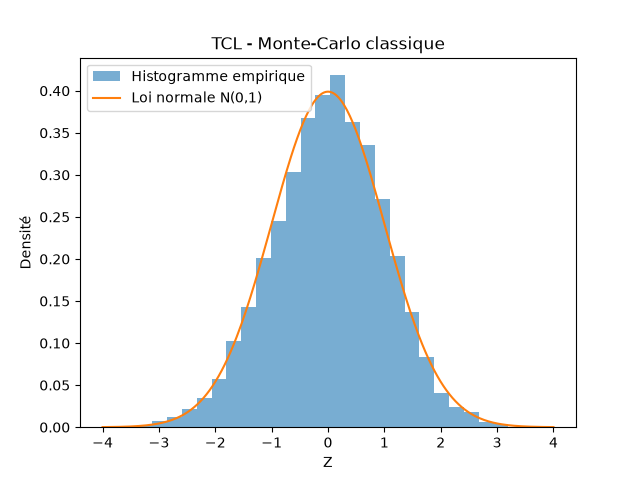
\includegraphics[width=0.8\textwidth]{TCL_montecarlo.png}
    \caption{Validation du TCL pour Monte-Carlo classique.}
    \label{fig:tcl-mc2}
\end{figure}

\begin{figure}[h]
    \centering
    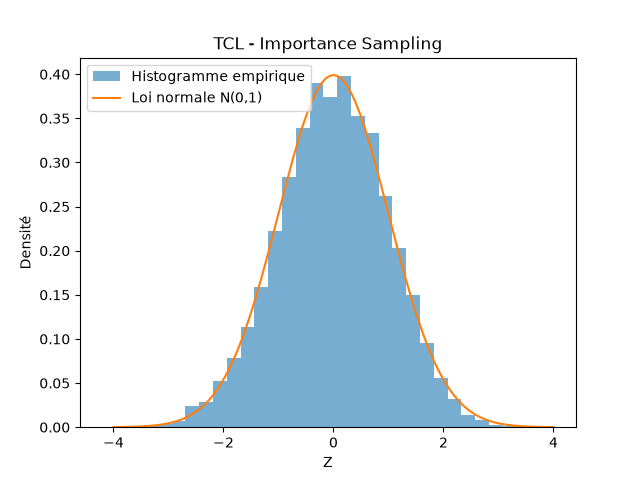
\includegraphics[width=0.8\textwidth]{TCL_IS.png}
    \caption{Validation du TCL pour l'échantillonnage d'importance.}
    \label{fig:tcl-is}
\end{figure}

Pour obtenir une même précision, le nombre de tirages nécessaires est
proportionnel à la variance de l'estimateur. Le rapport des budgets théoriques
est donc :
\[
\frac{N_{\mathrm{MC}}}{N_{\mathrm{IS}}}
=\frac{V_{\mathrm{MC}}}{V_{\mathrm{IS}}}
\approx 95{,}6.
\]
Ainsi, l'échantillonnage d'importance nécessite théoriquement environ 96 fois
moins d'échantillons pour obtenir une précision équivalente, sans tenir compte
du coût de génération des échantillons.

\subsection{Variance avec la densité d'importance optimale}

La densité d'importance optimale est :
\[
\widetilde q_{\mathrm{opt}}(x)
=\frac{g(x)q(x)}{\mu}
=\frac{\pi}{2}\cos\left(\frac{\pi x}{2}\right).
\]
Avec cette densité, le poids de l'estimateur est constant :
\[
\frac{g(x)q(x)}{\widetilde q_{\mathrm{opt}}(x)}
=\mu.
\]
L'estimateur vaut donc exactement $\mu$ pour chaque simulation. Les résultats
numériques donnent :
\[
\overline{\mu}=0{,}636620,
\qquad V_{\mathrm{emp}}=0.
\]
La variance est nulle, car la densité optimale nécessite de connaître $\mu$,
précisément la quantité à estimer. Elle est donc généralement inutilisable
directement.

\subsection{Importance sampling avec $\widetilde q(x)=2(1-x)$}

On considère la densité :
\[
\widetilde q(x)=2(1-x),\qquad x\in[0,1].
\]
Sa fonction de répartition est
\[
F(x)=\int_0^x 2(1-t)\,dt=2x-x^2.
\]
En posant $U=F(X)$ avec $U\sim\mathcal U([0,1])$, l'inversion de la fonction
de répartition donne :
\[
\boxed{X=1-\sqrt{1-U}.}
\]
La variance théorique de l'estimateur pour $N=50$ est :
\[
V_{\mathrm{IS}}\approx 1{,}35694\times10^{-4}.
\]
La simulation donne :
\[
\overline{\mu}_{\mathrm{emp}}=0{,}636706,
\qquad
V_{\mathrm{emp}}\approx 1{,}41963\times10^{-4}.
\]
Pour comparaison, la variance de Monte-Carlo classique est
$V_{\mathrm{MC}}\approx 1{,}89431\times10^{-3}$. La variance de cette méthode
d'importance est donc plus faible que celle de Monte-Carlo classique.

% ======================================================================
% PARTIE 2 : Filtrage particulaire
% ======================================================================

\section{Modèle}

\paragraph{État.} La pose du robot à l'instant $k$ est
$\X_k = (x_k, y_k, \theta_k)^\top \in \R^2 \times \left]-\pi,\pi\right]$.
On note $\wrap$ la fonction qui ramène un angle dans $\left]-\pi,\pi\right]$ et
$R(\theta)$ la rotation d'angle $\theta$.

\paragraph{Évolution.} Le déplacement $\uu_k = (\delta x, \delta y, \delta\theta)$
est exprimé dans le repère du robot. La pose suivante est obtenue par
composition de poses (fonction \texttt{tcomp}) :
\begin{equation}
  \X_k = f(\X_{k-1}, \uu_k) =
  \begin{pmatrix}
    x_{k-1} + \delta x \cos\theta_{k-1} - \delta y \sin\theta_{k-1}\\
    y_{k-1} + \delta x \sin\theta_{k-1} + \delta y \cos\theta_{k-1}\\
    \wrap(\theta_{k-1} + \delta\theta)
  \end{pmatrix}.
  \label{eq-f}
\end{equation}
La commande vraie est $\uu_k = \big(0,\ 0{,}1,\ 0{,}1\tfrac{\pi}{180}\sin(3\pi k/K)\big)$ :
le robot avance de $0{,}1$~m par pas avec un cap qui oscille lentement.

\paragraph{Odométrie.} Le robot ne connaît que la commande bruitée
\begin{equation}
  \tilde\uu_k = \uu_k + \bm\varepsilon_k, \qquad
  \bm\varepsilon_k \sim \N(0, Q), \qquad
  Q = \diag(0{,}02^2,\ 0{,}02^2,\ (1^\circ)^2).
\end{equation}
Intégrer seulement l'odométrie donne une erreur qui s'accumule : l'erreur de
cap est une marche aléatoire, et elle se transforme en erreur de position
proportionnelle à la distance parcourue.

\paragraph{Observation.} Il y a $20$ amers $\mathbf{m}_j$ placés au hasard dans
$[-60, 60]^2$. À chaque pas, le robot mesure la distance et l'angle relatif
d'un amer $j$ tiré au hasard :
\begin{equation}
  \z_k = h_j(\X_k) + \bm\eta_k, \qquad
  h_j(\X) =
  \begin{pmatrix}
    \sqrt{(m_{j,x} - x)^2 + (m_{j,y} - y)^2}\\
    \wrap\big(\operatorname{atan2}(m_{j,y} - y,\ m_{j,x} - x) - \theta\big)
  \end{pmatrix},
  \label{eq-h}
\end{equation}
avec $\bm\eta_k \sim \N(0, P_Y)$ et $P_Y = \diag(0{,}5^2,\ (1^\circ)^2)$. La fonction
$h_j$ est non linéaire : une seule mesure place le robot sur un cercle autour
de l'amer, donc la loi de $\X_k$ sachant les mesures n'est pas gaussienne en
général.

\paragraph{Bruits du filtre.} Le filtre utilise ses propres covariances
$Q_{\mathrm{est}}$ et $P_{Y,\mathrm{est}}$, égales par défaut à $2Q$ et $2P_Y$.

\section{Filtre particulaire}

\subsection{Filtrage bayésien}
On cherche la loi a posteriori $p(\X_k \mid \z_{1:k})$. Comme $(\X_k)$ est une
chaîne de Markov et que les mesures sont indépendantes sachant l'état, elle se
calcule récursivement en deux étapes.

\paragraph{Prédiction (Chapman--Kolmogorov).}
\begin{equation}
  p(\X_k \mid \z_{1:k-1}) = \int p(\X_k \mid \X_{k-1})\, p(\X_{k-1} \mid \z_{1:k-1})\, d\X_{k-1}.
  \label{eq-ck}
\end{equation}

\paragraph{Correction (Bayes).}
\begin{equation}
  p(\X_k \mid \z_{1:k}) =
  \frac{p(\z_k \mid \X_k)\, p(\X_k \mid \z_{1:k-1})}{\int p(\z_k \mid \X)\, p(\X \mid \z_{1:k-1})\, d\X}.
  \label{eq-bayes}
\end{equation}
Ces intégrales n'ont une solution exacte que dans le cas linéaire gaussien
(filtre de Kalman). Ici $f$ et $h_j$ sont non linéaires, donc on les approche
par Monte-Carlo.

\subsection{Approximation de Monte-Carlo}
Si $\X^{(1)}, \dots, \X^{(N)}$ sont tirés selon une loi $p$, alors
\begin{equation}
  \hat\mu_N = \frac1N \sum_{i=1}^N g(\X^{(i)}) \xrightarrow[N\to\infty]{p.s.} \E_p[g(\X)],
  \qquad
  \mathbb{V}(\hat\mu_N) = \frac{\mathbb{V}_p(g(\X))}{N}.
\end{equation}
L'erreur décroît donc en $1/\sqrt N$. On ne sait pas tirer directement selon
$p(\X_k \mid \z_{1:k})$ : on utilise l'échantillonnage d'importance. On tire
selon une densité $q$ et on corrige par des poids :
\begin{equation}
  \E_p[g(\X)] = \E_q\!\left[\frac{p(\X)}{q(\X)}\, g(\X)\right]
  \approx \sum_{i=1}^N w^{(i)} g(\X^{(i)}),
  \qquad w^{(i)} \propto \frac{p(\X^{(i)})}{q(\X^{(i)})},\quad \sum_i w^{(i)} = 1.
\end{equation}
La loi a posteriori est alors représentée par un nuage de particules pondérées
$\{\X_k^{(i)}, w_k^{(i)}\}$.

\subsection{Filtre bootstrap}
\begin{proposition}
Si on prend comme densité d'importance la dynamique,
$q(\X_k \mid \X_{k-1}^{(i)}) = p(\X_k \mid \X_{k-1}^{(i)})$, alors les poids se
mettent à jour par
\begin{equation}
  w_k^{(i)} \propto w_{k-1}^{(i)}\, p(\z_k \mid \X_k^{(i)}).
  \label{eq-poids}
\end{equation}
\end{proposition}
\begin{proof}
Pour une trajectoire, la cible vérifie
\[
p(\X_{0:k} \mid \z_{1:k}) \propto p(\z_k \mid \X_k)\, p(\X_k \mid \X_{k-1})\, p(\X_{0:k-1} \mid \z_{1:k-1})
\]
et la densité d'importance est $q(\X_{0:k}) = p(\X_k \mid \X_{k-1})\, q(\X_{0:k-1})$.
Le rapport des deux donne
$w_k \propto \dfrac{p(\z_k \mid \X_k)\, p(\X_k \mid \X_{k-1})}{p(\X_k \mid \X_{k-1})}\, w_{k-1}
= p(\z_k \mid \X_k)\, w_{k-1}$.
\end{proof}
La prédiction~\eqref{eq-ck} se fait donc en simulant chaque particule avec
le modèle d'évolution, et la correction~\eqref{eq-bayes} en multipliant les
poids par la vraisemblance.

\paragraph{Dégénérescence et rééchantillonnage.} Avec~\eqref{eq-poids}, la
variance des poids augmente avec $k$ et, au bout de quelques pas, une seule
particule porte presque tout le poids. On le mesure par la taille effective
\begin{equation}
  \Neff = \frac{1}{\sum_{i=1}^N (w_k^{(i)})^2} \in [1, N],
\end{equation}
qui vaut $N$ si les poids sont égaux et $1$ si une particule a tout le poids.
Le rééchantillonnage tire $N$ particules parmi les anciennes avec probabilités
$w_k^{(i)}$ (les lourdes sont dupliquées, les légères éliminées) puis remet
les poids à $1/N$. Le code le fait à chaque pas ; le filtre SIR ne le fait que si
$\Neff < \theta N$.

\paragraph{Estimation.} On utilise la moyenne et la covariance pondérées
\begin{equation}
  \hat\X_k = \sum_i w_k^{(i)} \X_k^{(i)}, \qquad
  \hat P_k = \sum_i w_k^{(i)} (\X_k^{(i)} - \hat\X_k)(\X_k^{(i)} - \hat\X_k)^\top .
\end{equation}

\subsection{Cas du robot}
Dans le code, les étapes deviennent :
\begin{enumerate}
  \item \textbf{Initialisation :}
  $\X_0^{(i)} = \X_0 + \diag(1, 1, 0{,}1)\,\bm\xi^{(i)}$, $\bm\xi^{(i)} \sim \N(0, I_3)$
  (écarts-types $1$~m, $1$~m, $0{,}1$~rad).
  \item \textbf{Prédiction :}
  $\X_k^{(i)} = f\big(\X_{k-1}^{(i)},\ \tilde\uu_k + \mathbf{v}^{(i)}\big)$ avec
  $\mathbf{v}^{(i)} \sim \N(0, Q_{\mathrm{est}})$.
  \item \textbf{Correction :} innovation
  $\bm\nu^{(i)} = \z_k - h_j(\X_k^{(i)})$ (angle ramené dans $\left]-\pi,\pi\right]$),
  puis
  \begin{equation}
    w^{(i)} \propto \exp\!\Big(-\tfrac12\, \bm\nu^{(i)\top} P_{Y,\mathrm{est}}^{-1}\, \bm\nu^{(i)}\Big) + 10^{-3}.
  \end{equation}
  La constante de la gaussienne disparaît à la normalisation. Comme on
  rééchantillonne à chaque pas, $w_{k-1}^{(i)} = 1/N$ et~\eqref{eq-poids} se
  réduit à la vraisemblance. Le terme $10^{-3}$ évite que tous les poids
  soient nuls.
  \item \textbf{Estimation} de $\hat\X_k$ et $\hat\sigma_x = \sqrt{(\hat P_k)_{11}}$,
  puis \textbf{rééchantillonnage} à faible variance.
\end{enumerate}

\paragraph{Protocole.} Toutes les expériences utilisent $K = 2000$ pas, la même
carte et les mêmes mesures (graine fixée), et sauf mention contraire $N = 1000$
et les réglages du code. On regarde l'erreur sur $x$, $e_x = \hat x_k - x_k$,
et l'enveloppe $\pm 3\hat\sigma_x$ donnée par le filtre : si le filtre est
cohérent, l'erreur doit rester dans l'enveloppe. Tout le code est dans
\texttt{tp\_filtre\_particulaire.py}.

\begin{figure}[h]
  \centering
  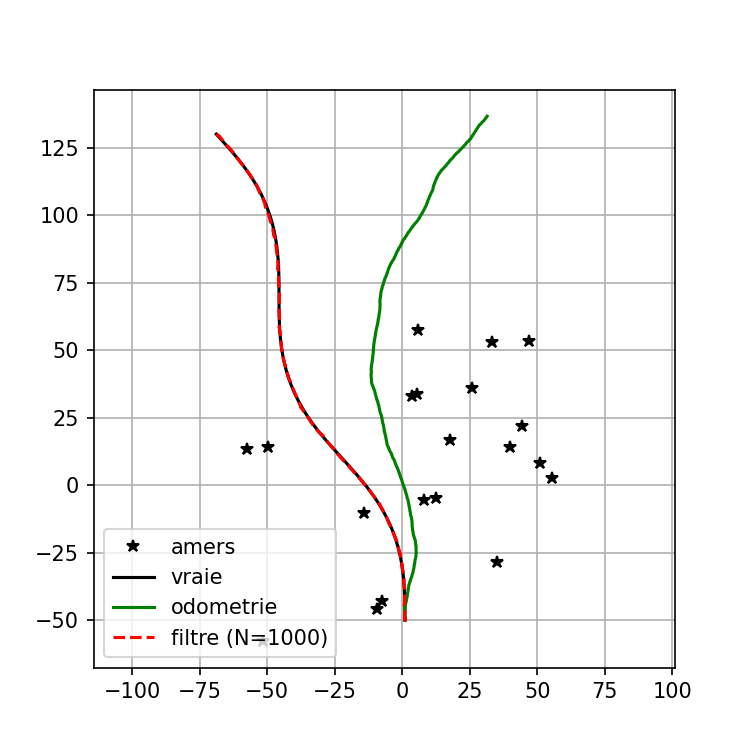
\includegraphics[width=0.42\textwidth]{scenario.png}
  \caption{Scénario : amers, trajectoire vraie, odométrie et estimée du filtre.}
  \label{fig-scenario}
\end{figure}

\section{Nombre de particules}

\begin{figure}[h]
  \centering
  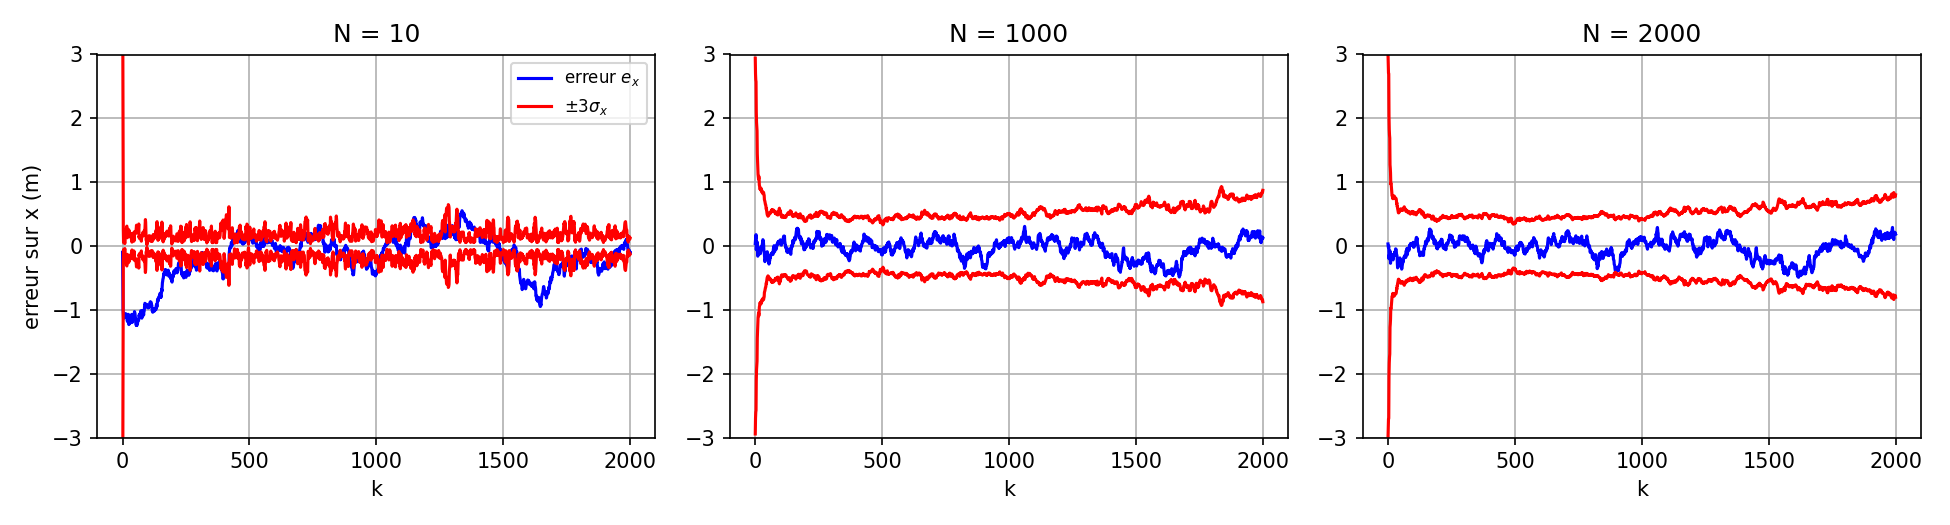
\includegraphics[width=\textwidth]{nparticles.png}
  \caption{Erreur $e_x$ et enveloppe $\pm3\hat\sigma_x$ pour $N = 10$, $1000$, $2000$.}
  \label{fig-N}
\end{figure}

\begin{table}[h]
  \centering
  \begin{tabular}{rccc}
    \toprule
    $N$ & moyenne $|e_x|$ (m) & variance $e_x$ (m$^2$) & temps (s) \\
    \midrule
    10   & 0,294 & 0,129 & 0,3 \\
    500  & 0,126 & 0,025 & 10,4 \\
    1000 & 0,120 & 0,023 & 20,7 \\
    1500 & 0,127 & 0,026 & 30,9 \\
    2000 & 0,123 & 0,024 & 41,2 \\
    \bottomrule
  \end{tabular}
  \caption{Erreur et temps de calcul en fonction de $N$.}
  \label{tab-N}
\end{table}

Avec $N = 10$, l'erreur est grande et sort souvent de l'enveloppe : le filtre
annonce une incertitude trop petite (\cref{fig-N}). Avec si peu de
particules, le rééchantillonnage duplique toujours les mêmes et le nuage perd
sa diversité. À partir de $N = 500$, l'erreur ne diminue presque plus
(\cref{tab-N}) : elle est limitée par le bruit des capteurs et non plus par
l'approximation de Monte-Carlo, dont l'erreur en $1/\sqrt N$ devient
négligeable. Les courbes pour $N = 1000$ et $N = 2000$ sont presque
identiques, alors que le temps de calcul est proportionnel à $N$. Quelques
centaines de particules suffisent donc dans ce scénario.

\section{Variance initiale}

On multiplie les écarts-types du nuage initial par un facteur $s$, et on
considère deux cas :
\begin{itemize}
  \item \textbf{cas A} : le nuage est centré sur la vraie pose $\X_0$, comme
  dans le code fourni ;
  \item \textbf{cas B} : le nuage est centré sur une estimée fausse
  $\X_0 + (3,\ -3,\ 0{,}3)$, ce qui est plus réaliste.
\end{itemize}
On teste aussi une initialisation uniforme sur toute la carte (localisation
globale).

\begin{figure}[h]
  \centering
  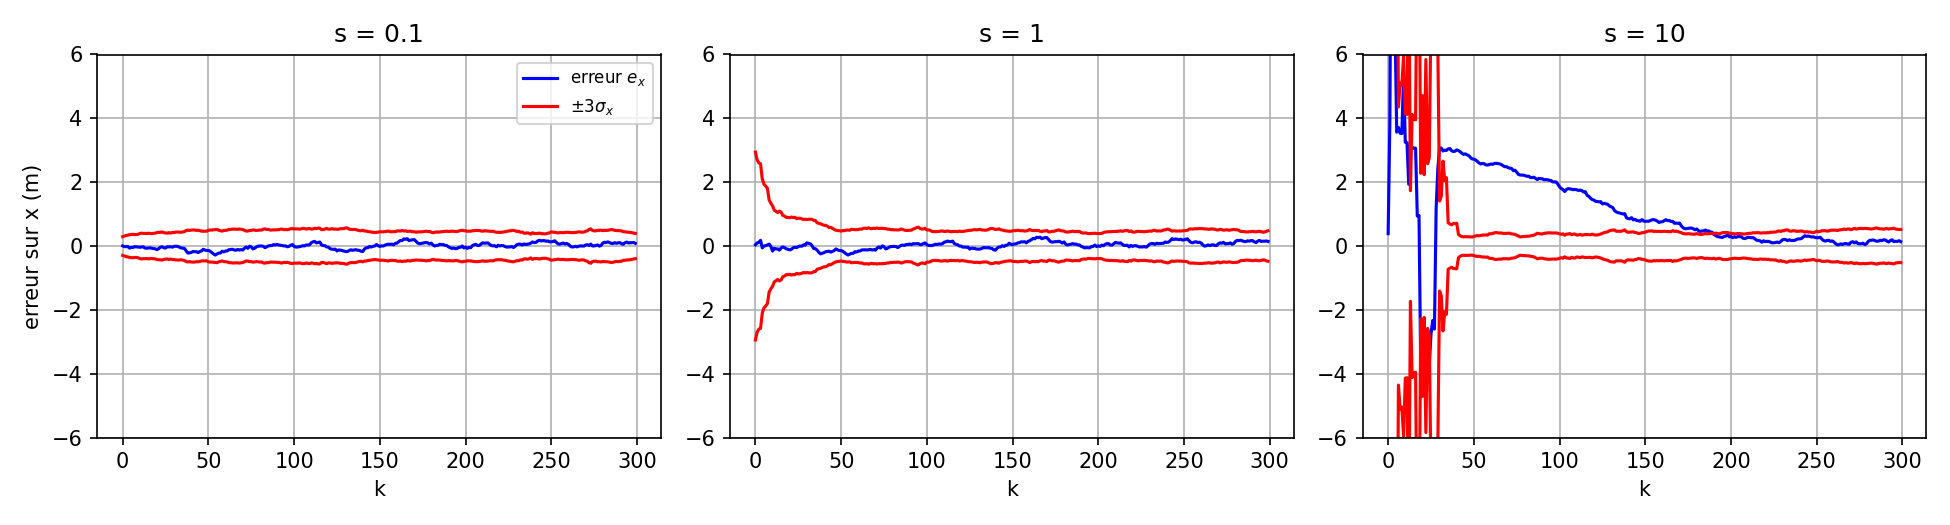
\includegraphics[width=\textwidth]{init_A.png}\\[0.3em]
  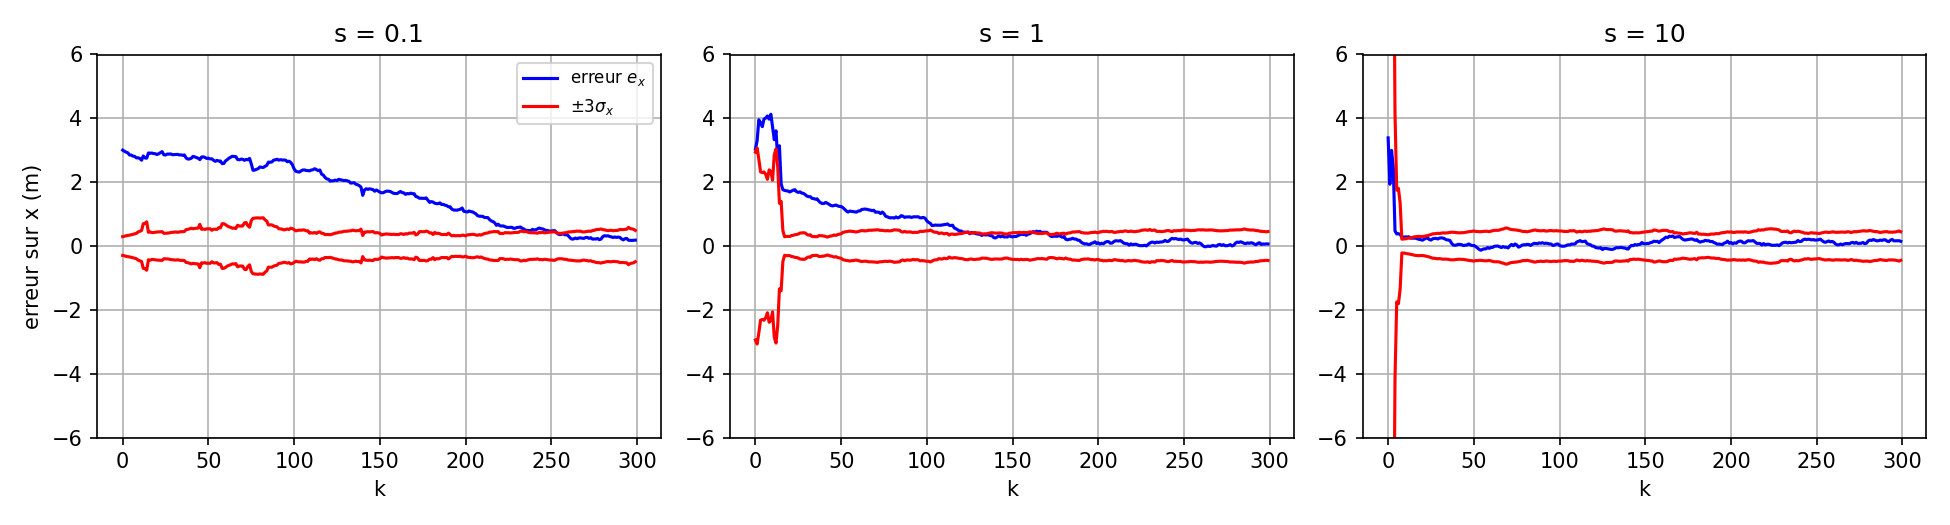
\includegraphics[width=\textwidth]{init_B.png}
  \caption{Nuage initial d'écart-type $s \cdot \diag(1, 1, 0{,}1)$, 300 premiers
  pas. Haut : cas A (centré sur $\X_0$). Bas : cas B (centré sur
  $\X_0 + (3, -3, 0{,}3)$).}
  \label{fig-init}
\end{figure}

\begin{table}[h]
  \centering
  \begin{tabular}{c c ccc}
    \toprule
    cas & nuage initial & moyenne $|e_x|$ (m) & max $|e_x|$ (m) & $|e_x|$ final (m) \\
    \midrule
    A & $s = 0{,}1$ & 0,11 & 0,4  & 0,15 \\
    A & $s = 1$     & 0,12 & 0,5  & 0,13 \\
    A & $s = 10$    & 0,30 & 13,7 & 0,10 \\
    A & $s = 50$    & 10,3 & 31,2 & 14,4 \\
    \midrule
    B & $s = 0{,}1$ & 0,36 & 3,0  & 0,26 \\
    B & $s = 1$     & 0,21 & 4,1  & 0,18 \\
    B & $s = 10$    & 0,13 & 3,4  & 0,05 \\
    B & $s = 50$    & 84,9 & 192,8 & 192,8 \\
    \midrule
    -- & uniforme   & 4,24 & 19,1 & 0,22 \\
    \bottomrule
  \end{tabular}
  \caption{Influence de la dispersion du nuage initial ($N = 1000$).}
  \label{tab-init}
\end{table}

\paragraph{Cas A.} Quand le nuage est centré sur la vraie pose, un petit nuage
est le meilleur choix : pour $s = 0{,}1$ et $s = 1$ l'erreur est faible dès le
départ (\cref{fig-init}, haut). Le filtre connaît déjà la bonne position et
n'a rien à chercher. Avec $s = 10$, les particules sont dispersées sur
plusieurs dizaines de mètres et peu d'entre elles sont proches de la vérité :
l'estimée saute pendant les premiers pas (erreur jusqu'à $13{,}7$~m), puis se
recale lentement. Avec $s = 50$, le filtre se perd.

\paragraph{Cas B.} Quand le nuage est centré à côté de la vraie pose, la
conclusion change. Si le nuage est trop petit ($s = 0{,}1$ ou $1$), il ne
contient pas la vraie position. Toutes les particules ont une vraisemblance
très faible, les poids sont presque égaux et les mesures corrigent peu :
l'erreur de $3$~m ne diminue que lentement, en $150$ à $250$ pas, grâce au
bruit $Q_{\mathrm{est}}$ qui étale le nuage (\cref{fig-init}, bas). Pendant ce
temps, le filtre est trop confiant : l'erreur est très au-dessus de
l'enveloppe. Avec $s = 10$, le nuage couvre la vraie position et le filtre se
recale en quelques pas. Avec $s = 50$, le filtre se perd complètement.

\paragraph{Localisation globale.} Avec le nuage uniforme, le filtre fait de
grandes erreurs au début (jusqu'à $19$~m) mais finit par trouver le robot pour
cette simulation ($0{,}22$~m d'erreur finale). Ce résultat dépend du hasard :
avec $1000$ particules sur toute la carte, très peu sont compatibles avec les
premières mesures, et le filtre peut aussi se fixer sur une mauvaise position.

La dispersion initiale doit donc représenter l'incertitude réelle sur la pose
de départ : petite si on la connaît bien (cas A), assez grande pour couvrir
l'erreur si on la connaît mal (cas B), mais jamais trop grande pour le nombre
de particules.

\section{Bruits du filtre}

On pose $Q_{\mathrm{est}} = \alpha_Q\, Q$ et $P_{Y,\mathrm{est}} = \alpha_R\, P_Y$ :
$\alpha < 1$ signifie que le filtre sous-estime le bruit, $\alpha = 1$ qu'il le
connaît exactement, $\alpha > 1$ qu'il le surestime. On fait varier un seul
facteur, l'autre restant à $2$.

\begin{figure}[h]
  \centering
  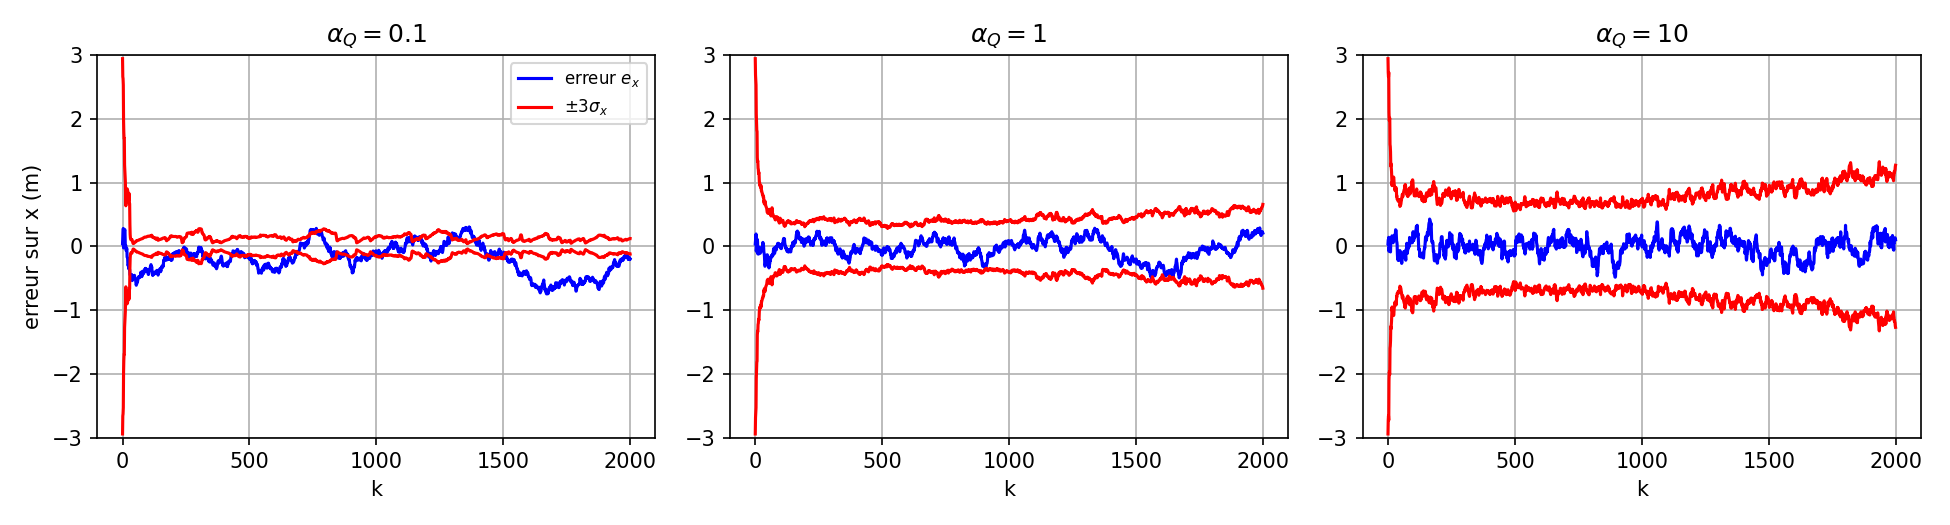
\includegraphics[width=\textwidth]{bruit_Q.png}\\[0.3em]
  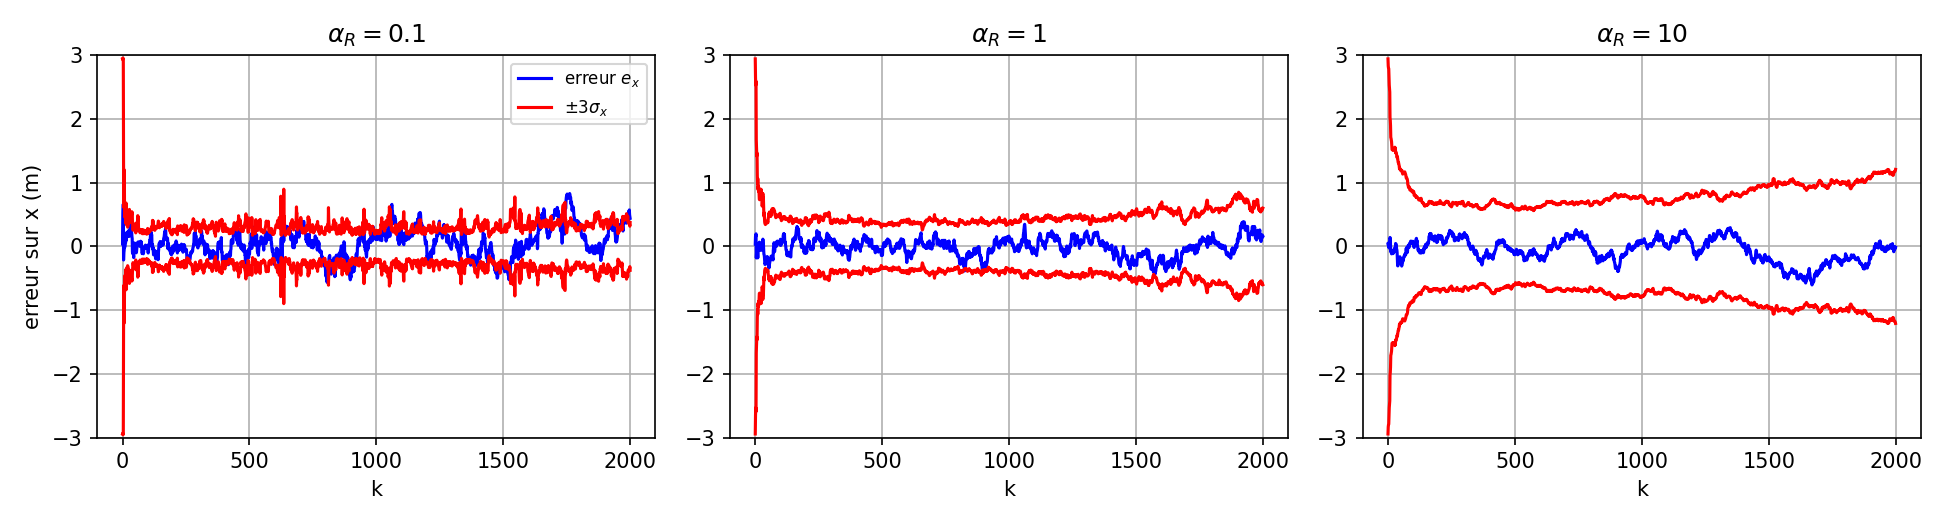
\includegraphics[width=\textwidth]{bruit_R.png}
  \caption{Bruit de mouvement (haut) et de mesure (bas) sous-estimé, exact ou surestimé.}
  \label{fig-bruits}
\end{figure}

\begin{table}[h]
  \centering
  \begin{tabular}{c cc cc}
    \toprule
    & \multicolumn{2}{c}{$\alpha_Q$ varie} & \multicolumn{2}{c}{$\alpha_R$ varie} \\
    \cmidrule(lr){2-3}\cmidrule(lr){4-5}
    $\alpha$ & moy.\ $|e_x|$ (m) & moy.\ $\hat\sigma_x$ (m) & moy.\ $|e_x|$ (m) & moy.\ $\hat\sigma_x$ (m) \\
    \midrule
    0,1 & 0,253 & 0,051 & 0,188 & 0,107 \\
    1   & 0,128 & 0,152 & 0,113 & 0,156 \\
    2   & 0,120 & 0,184 & 0,120 & 0,184 \\
    10  & 0,121 & 0,275 & 0,157 & 0,276 \\
    \bottomrule
  \end{tabular}
  \caption{Erreur moyenne et écart-type annoncé selon les bruits du filtre.}
  \label{tab-bruits}
\end{table}

\paragraph{Bruit de mouvement.} Avec $\alpha_Q = 0{,}1$, le nuage ne s'étale
pas assez pour suivre la dérive réelle de l'odométrie. L'erreur double et
sort souvent de l'enveloppe, qui est trop étroite (\cref{fig-bruits}, haut).
Avec $\alpha_Q = 10$, l'erreur ne change presque pas, mais le nuage est trop
large : le filtre reste cohérent avec une enveloppe beaucoup trop grande.

\paragraph{Bruit de mesure.} Avec $\alpha_R = 0{,}1$, la vraisemblance est trop
étroite : seules quelques particules gardent du poids et l'estimée suit le bruit
de chaque mesure. L'erreur augmente et l'enveloppe est trop petite. Avec
$\alpha_R = 10$, les mesures comptent moins, l'erreur augmente légèrement et
l'enveloppe est beaucoup trop large.

Sous-estimer un bruit rend donc le filtre trop confiant ; le surestimer le
rend prudent mais robuste. Les réglages $\alpha = 1$ et $\alpha = 2$ (choix
du code) donnent des erreurs très proches ; $\alpha = 2$ garde une marge de
sécurité si les bruits réels sont mal connus.

\section{Panne capteur}

On supprime les mesures pour $400 < k < 500$. Pendant la panne, le filtre ne
fait que la prédiction~\eqref{eq-ck} : la loi a posteriori s'élargit à chaque
pas et seul $Q_{\mathrm{est}}$ fixe la vitesse de cet élargissement.

\begin{figure}[h]
  \centering
  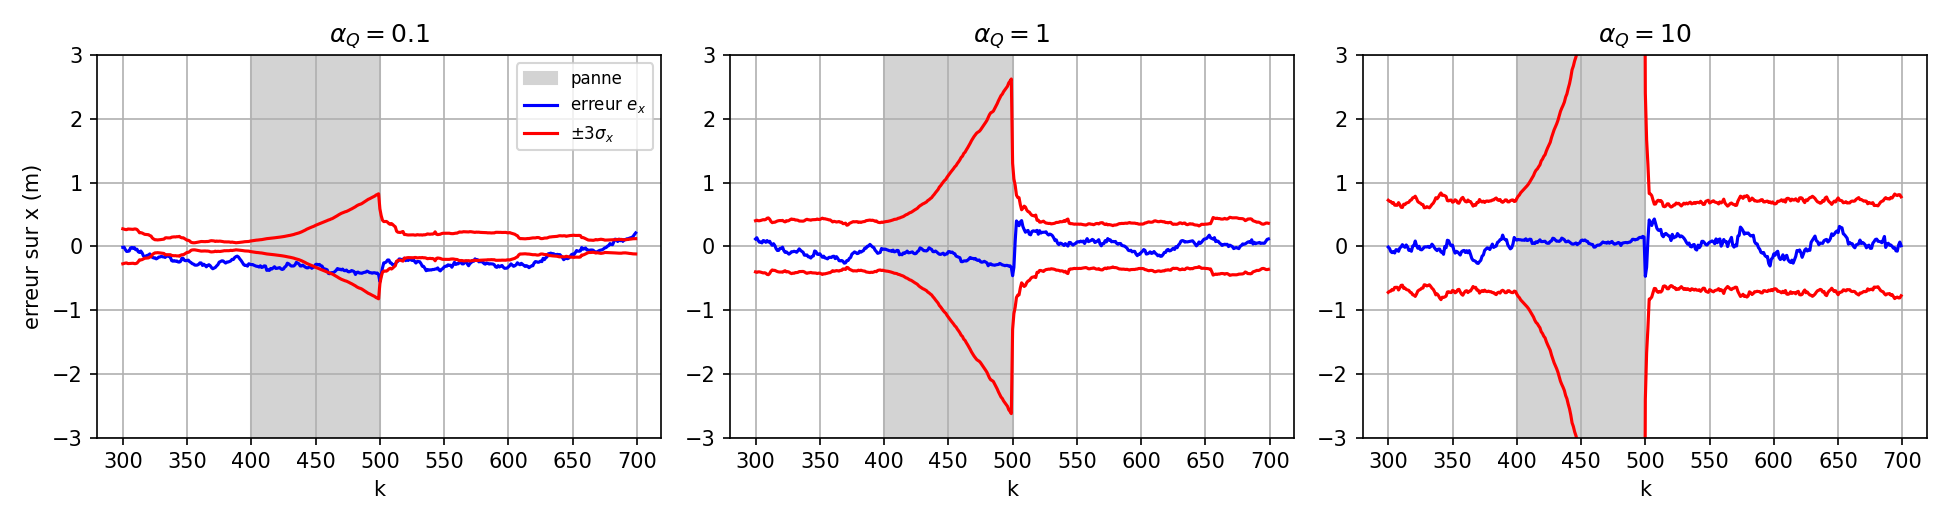
\includegraphics[width=\textwidth]{panne.png}
  \caption{Panne capteur (zone grise) pour $\alpha_Q = 0{,}1$, $1$, $10$.}
  \label{fig-panne}
\end{figure}

\begin{table}[h]
  \centering
  \begin{tabular}{cccc}
    \toprule
    $\alpha_Q$ & max $|e_x|$ pendant (m) & $3\hat\sigma_x$ en fin de panne (m) & max $|e_x|$ après (200 pas) \\
    \midrule
    0,1 & 0,45 & 0,82 & 0,55 \\
    1   & 0,33 & 2,62 & 0,46 \\
    10  & 0,16 & 7,58 & 0,47 \\
    \bottomrule
  \end{tabular}
  \caption{Comportement pendant et après la panne $400 < k < 500$.}
  \label{tab-panne}
\end{table}

Dans les trois cas, l'erreur reste inférieure à $0{,}5$~m : l'odométrie dérive
peu pendant ces $100$ pas. La différence est dans l'enveloppe, qui s'ouvre
pendant la panne puis se referme dès le retour des mesures (\cref{fig-panne}).
Avec $\alpha_Q = 0{,}1$, elle s'ouvre trop peu et l'erreur en sort : le filtre
se croit précis alors qu'il n'a plus de mesures, et il est un peu moins bon
après la panne. Avec $\alpha_Q = 10$, elle s'ouvre beaucoup trop ($7{,}6$~m pour
une erreur de $0{,}2$~m) et la première mesure après la panne provoque un saut de
l'estimée. Le modèle exact $\alpha_Q = 1$ donne une incertitude qui grandit de
façon réaliste et un recalage rapide.

\section{Filtre SIR}

On garde maintenant les poids d'un pas à l'autre avec~\eqref{eq-poids} et on
ne rééchantillonne que si $\Neff < \theta N$.

\begin{figure}[h]
  \centering
  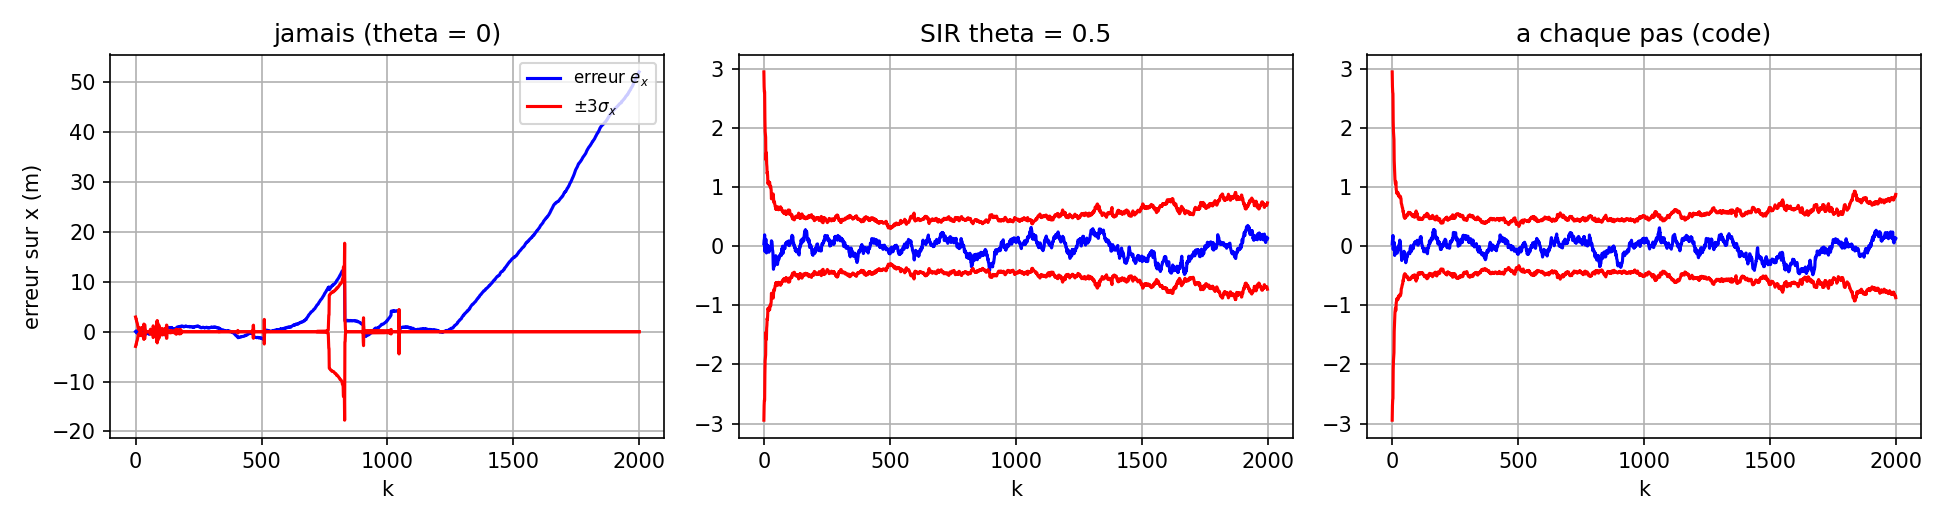
\includegraphics[width=\textwidth]{sir.png}
  \caption{Sans rééchantillonnage, SIR avec $\theta = 0{,}5$, et rééchantillonnage à chaque pas.}
  \label{fig-sir}
\end{figure}

\begin{table}[h]
  \centering
  \begin{tabular}{lccc}
    \toprule
    rééchantillonnage & moyenne $|e_x|$ (m) & max $|e_x|$ (m) & nombre \\
    \midrule
    jamais ($\theta = 0$)  & 10,2  & 52,1 & 0 \\
    SIR $\theta = 0{,}5$   & 0,124 & 0,48 & 943 \\
    à chaque pas     & 0,120 & 0,49 & 1999 \\
    \bottomrule
  \end{tabular}
  \caption{Influence du rééchantillonnage.}
  \label{tab-sir}
\end{table}

Sans rééchantillonnage, les poids dégénèrent en quelques pas : une seule
particule porte tout le poids, l'enveloppe devient nulle et l'estimée dérive
comme une odométrie, jusqu'à $52$~m d'erreur (\cref{fig-sir}). Le rééchantillonnage est donc
indispensable. Le SIR avec $\theta = 0{,}5$ donne presque la même précision que
le code fourni avec deux fois moins de rééchantillonnages
(\cref{tab-sir}). Rééchantillonner à chaque pas n'est donc pas nécessaire :
cela coûte du calcul et réduit inutilement la diversité du nuage quand les
poids sont encore équilibrés. Le SIR évite aussi de rééchantillonner pendant
une panne, où les poids ne changent pas.

\section{Conclusion}

Ce TP a mis en évidence deux usages complémentaires des méthodes de Monte-Carlo.
Pour l'intégration, l'échantillonnage d'importance réduit fortement la variance
de l'estimateur dès lors que la densité d'importance est bien choisie, ce qui
diminue d'autant le nombre de tirages nécessaires pour une précision donnée.
Pour la localisation, le filtre particulaire approxime la loi a posteriori par
un nuage de particules pondérées : quelques centaines suffisent, le nuage
initial doit refléter l'incertitude réelle et il vaut mieux surestimer que
sous-estimer les bruits. Dans les deux cas, la qualité du résultat repose sur
un bon choix de densité d'importance ou de proposition.

\end{document}
